\section{History}
eBay was founded 1995 in San Jose (CA) as AuctionWeb by Pierre Omidyar. One year later, eBay bought a third-party licence from Electronic Travel Auction to sell plane tickets and other travelling stuff. During the year 1996, over 200'000 auctions were available on the website. At the beginning of 1997 the number of auctions exploded (about 2 million articles). In the same year the company get their well-known name eBay and received 6.7 million dollar from the venture capital firm Benchmark Capital. The company went public on the stock exchange on September 21, 1998 and the share price increased from 18 to 53.5 dollar on the first day of trading. Four years later the growth continues and eBay bought the online money transfer service PayPal. eBay expanded worldwide in early 2008, had hundred millions of registered users and 15'000 employees. Today, the firm is one of the world's largest online marketplaces. During the fourth quarter of the year 2013 about 128 million active users were reported. A cell phone was sold every 4 seconds, a pair of shoes every 2 seconds and a Ford Mustang every 55 minutes.

\section{Auction item composition}
Every eBay user has the possibility to create auctions for different kind of items. To present the article, the seller has to provide accurate information about it. The standard eBay auction consists of the following fields:
\begin{itemize}
	\item \textbf{Title} The title of the item is limited to 80 characters. The sellers should use descriptive keywords to clearly and accurately convey what they are selling
	\item \textbf{Description} The description is the opportunity to provide the buyers with more information about the item
	\item \textbf{Category} An item can have multiple predefined categories. eBay provides a list of categories which the seller can select
	\item \textbf{Condition} The condition of the item is dependent on the selected category. eBay provides different condition schemas. For clothing items the seller can select between 'New with tags', 'New without tags', 'New with defects' or 'Pre-owned'. For other categories like books, other condition values are present: 'Brand new', 'Like new', 'Very good', 'Good', 'Acceptable'
	\item \textbf{Pictures} To visualise the item the auction creator can upload up to twelve pictures. The first image is important, because it appears next to the item's title in the search result. The pictures will be stored for 90 days on the eBay servers.
	\item \textbf{Shipping costs} The seller has to tell the future buyers how much shipping will cost. There are three possibilities:
	\begin{itemize}
		\item Free shipping
		\item Flat shipping, same cost to all buyers
		\item Shipping rate tables, eBay calculates the cost for every individual buyer dependent on the location
	\end{itemize}
	\item \textbf{Duration} An auction can have a duration of 1, 3, 5, 7 or 10 days. If the item has a fixed price, the auction is finished if a buyer is willing to pay this price.
	\item \textbf{Pricing} The seller can select a starting price and then the bidding will start at this price. A 'But it now' option is also available. The buyer can skip the bidding process.
	\item \textbf{Payment} The seller has to select the desired paying method like 'PayPal' or 'Payment upon pickup'
\end{itemize}

\section{APIs}
eBay provides multiple APIs for developing third party applications. This allows developers to search for auctions or create listings over the XML format. Three main interfaces are available:
\begin{figure}[h!]
\centering
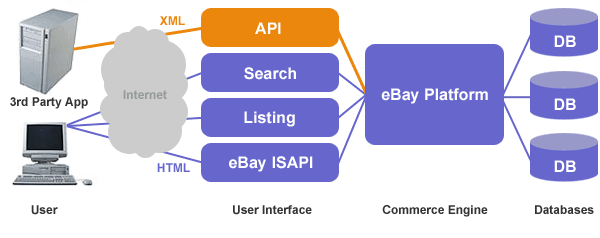
\includegraphics[scale=0.5]{images/api-flow.png}
\caption{eBay API overview}
\label{ebayAPI}
\end{figure}

\subsection{Trading API}
Developers use the Trading API to build applications such as selling and post-sales management applications, manage user information, and initiate the item purchase flow on eBay. The API is available in .NET, Java, PHP and Python.

\subsection{Shopping API}
The Shopping API provides a search engine for user information, popular items and reviews. The API is available in PHP and Python. Example calls for this API are:
\begin{itemize}
	\item \textit{findProducts()}: Search for products by keywords or ProductId
	\item \textit{GetSingleItem()}: Buyer specific view of an item
	\item \textit{GetUserProfile()}: Get the user profile and feedback information
\end{itemize}

\subsection{Finding API}
The Finding API provides access to the next generation search capabilities on the eBay platform. The developer can search and browse for items based on keyword queries, categories or an image. The API is available in .NET, Java and Python. Example calls for this API are:
\begin{itemize}
	\item \textit{findCompletedItems()}: Find the items which are listened as completed or no longer available on eBay
	\item \textit{findItemsByCategory()}: Find items in a specific category
	\item \textit{findItemsByImage()}: Find items which have a high similarity to a given image
\end{itemize}

\subsection{Example}
The following listing in Python illustrate the functionality of the Finding API. The developer has to register to the eBay developers program first. After that, a application ID can be created. This is necessary to get access to the eBay databases. A functioning Python environment and the additional eBay Python SDK are requirements to successfully execute the example
\lstset{language=Python,caption={eBay Finding API example},label=findingapi_example}
\begin{lstlisting}
from ebaysdk.finding import Connection as Finding
from ebaysdk.exception import ConnectionError
import json

try:
    api = Finding(appid='Universi-3c25-4b4e-b3e6-8c2568808b12')
    api.execute('findCompletedItems', {
        'keywords': 'ford mustang',
        'itemFilter': [
            {'name': 'ListingType',
             'value': 'Auction'},
            {'name': 'Currency',
             'value': 'USD'},                
            {'name': 'SoldItemsOnly',
             'value': 'true'},                 
        ],        
        'sortOrder': 'StartTimeNewest',
        })
    response = json.loads(api.response_json())
    
    print response['searchResult']['item'][0]
    
except ConnectionError as e:
    raise e  
\end{lstlisting}
The initialisation of the application is done on line 6. A correct application ID is required. Then the API call \textit{findCompletedItems()} is executed with some keywords and filter options. Only the newest auctions with at least one bidder and a payment in US dollar will be returned. The function \textit{response\_json()} (on line 19) returns the first 100 items by default. At the end, the first result will be printed to the console. Here is a shorter simplified version with the most important fields of the output:
\begin{table}[h!]
	\begin{center}
	\begin{tabular}{| l | l |}
		\hline
		\textbf{Name} & \textbf{Value} \\
		\hline
		itemId & 281273507096 \\
		\hline
		title & 2014 Hot Wheels Super Treasure Hunt 71 Mustang Mach 1 \\
		\hline
		categoryName & Diecast-Modern Manufacture \\
		\hline
		shippingType & Calculated \\
		\hline
		currentPrice & 18.5 USD \\
		\hline
		bidCount & 1 \\
		\hline
		paymentMethod & PayPal \\
		\hline
		conditionDisplayName & New \\
		\hline
		startTime & 2014-02-25T04:32:17.000Z \\
		\hline
		endTime & 2014-02-25T05:27:14.000Z \\
		\hline
	\end{tabular}
	\end{center}
	\caption{eBay Finding API example output}
\end{table}
